%==============================================================================
% locality-performance.tex
%==============================================================================

\chapter{Performance Evaluation}
\label{chap:locality-performance}

This chapter presents our performance evaluation of LASSI. First we
compare the performance of locality-ignorant benchmarks run with LASSI
and the original scheduler implementation. It is important that
LASSI's performance is comparable to that of the original
scheduler. Then we study different locality-aware benchmarks. By
scheduling data sharing intervals on the same processor they perform
prefetching of shared regions for one another which improves
performance. Our locality-aware benchmarks only explore data sharing
intervals and do not test how scheduling non-communicating intervals
with high memory footprints on different processors could help in
reducing cache contention and potential cache capacity problems.

\section{Methodology}
\label{sec:locality-performance-methodology}

The performance results in this chapter are obtained on an Intel
Nehalem system with 2 processors and 8 cores, running Ubuntu 9.04
64-bit with kernel 2.6.29 patched to support perfmon2
\cite{Eranian2008} (Appendix
\ref{sec:experimental-setup-mafushi}). The JVM used is Sun Hotspot JDK
1.6.0\_20 which is invoked with the following parameters:

\begin{lstlisting}[style=Listing]
  -server -Xmx4096M -Xms4096M -Xss8M -XX:+UseNUMA
\end{lstlisting}

Besides the runtime of the benchmarks, we are mostly interested in the
count of cache hit and miss events. Since the last level cache is part
of the uncore, we have to use the uncore PMU to count L3 cache
events. We use perfmon2 to track the following events
\cite{Levinthal2009}:

\begin{itemize}
\item \lstinline!UNC_LLC_HITS.READ!: Number of L3 cache read hits
\item \lstinline!UNC_LLC_MISS.READ!: Number of L3 cache read misses
\end{itemize}

The number of cache read hits and misses can also be determined by
tracking requests being sent to the uncore's Global Queue, but it is
simpler with the events listed above.

The execution times and cache events counts reported are the average
of the 3 best benchmark iterations from 10 separate invocations.


\section{Non-Locality Benchmarks}
\label{sec:locality-performance-non-locality}

It is important that our new scheduler implementation does not affect
the performance of existing locality-ignorant intervals
applications. Thus, we run the locality-ignorant JGF benchmarks
(Appendix \ref{chap:benchmarks}) with our new scheduler
implementation. As Figure \ref{fig:locality-performance-jgf} shows,
the performance of the locality-ignorant JGF benchmarks executed on
LASSI is comparable to the original implementation.

\begin{figure}[!ht]
  \centering
  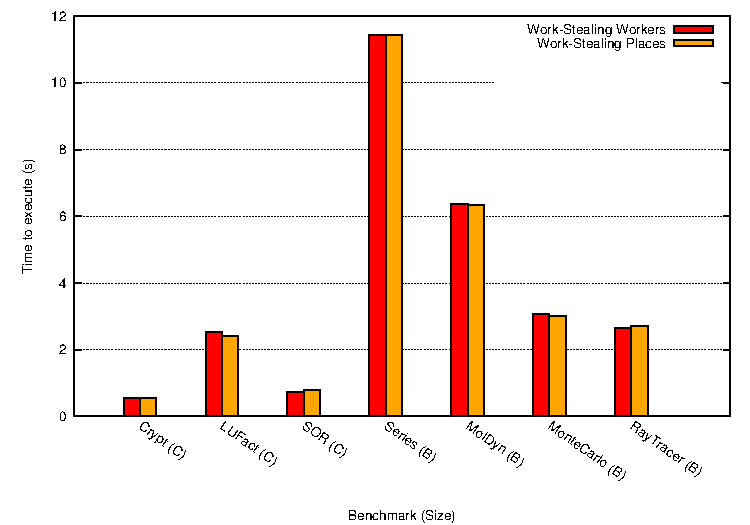
\includegraphics[width=0.8\linewidth]{locality-performance/mafushi-jgf}
  \caption[Locality-ignorant JGF benchmarks]{Locality-ignorant JGF
    benchmarks using LASSI on our Intel Nehalem (Appendix
    \ref{sec:experimental-setup-mafushi}) test machine}
  \label{fig:locality-performance-jgf}
\end{figure}


\section{Locality Benchmarks}
\label{sec:locality-performance-locality}

\subsection{Cache-Stress Test}
\label{sec:locality-performance-cache-stress-test}

We ported the \emph{Cache Stress Test} benchmark from the threaded
version developed in Chapter \ref{chap:locality-approach} to use
intervals.

Like the threaded version, it first randomly initializes two integer
arrays of equal size to the last level cache per processor. Then it
creates an inline root interval which produces 64 subintervals with
their locality set to a specific place: 32 have their locality set for
\emph{place 0} and 32 for \emph{place 1}.

One half of the subintervals operate on the elements of the first
array and the other half operate on the elements of the second
array. Each interval's task adds and multiplies all the elements of
its respective array 100 times.

Like in the threaded version, we implement several different variants
of the benchmark, each having different locality properties:

\begin{description}
\item[Best Locality:] All the intervals working on the first array
  have their locality set to \emph{place 0} and all intervals working
  on the second array have their locality set to \emph{place 1}.
\item[Ignorant Locality:] The intervals do not have any locality set,
  i.e. they are locality-ignorant.
\item[Random Locality:] The locality of the intervals is set to a
  \emph{random} place.
\item[Worst Locality:] Half the intervals with locality for
  \emph{place 0} work on the first array, and the other half work on
  the second array and vice versa for the intervals with locality for
  \emph{place 1}.
\end{description}

Figure \ref{fig:locality-performance-cache-stress-test-mafushi} shows
the place allocations for the benchmark variants with \emph{best} and
\emph{worst locality}.

\begin{figure}[!ht]
  \centering
  \subfloat[Best Locality]{
    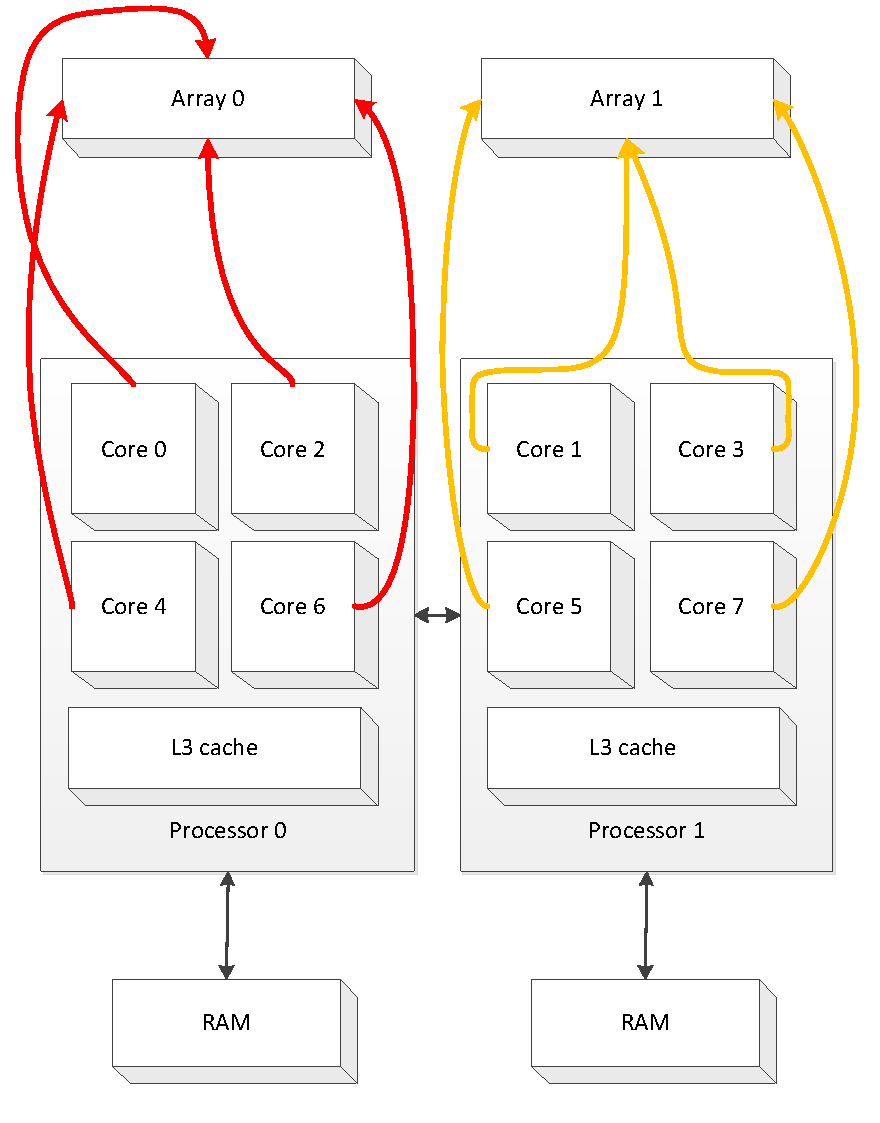
\includegraphics[width=0.5\linewidth]{locality-performance/cache-stress-test-mafushi-best}
    \label{fig:locality-performance-cache-stress-mafushi-best}
  }
  \subfloat[Worst Locality]{
    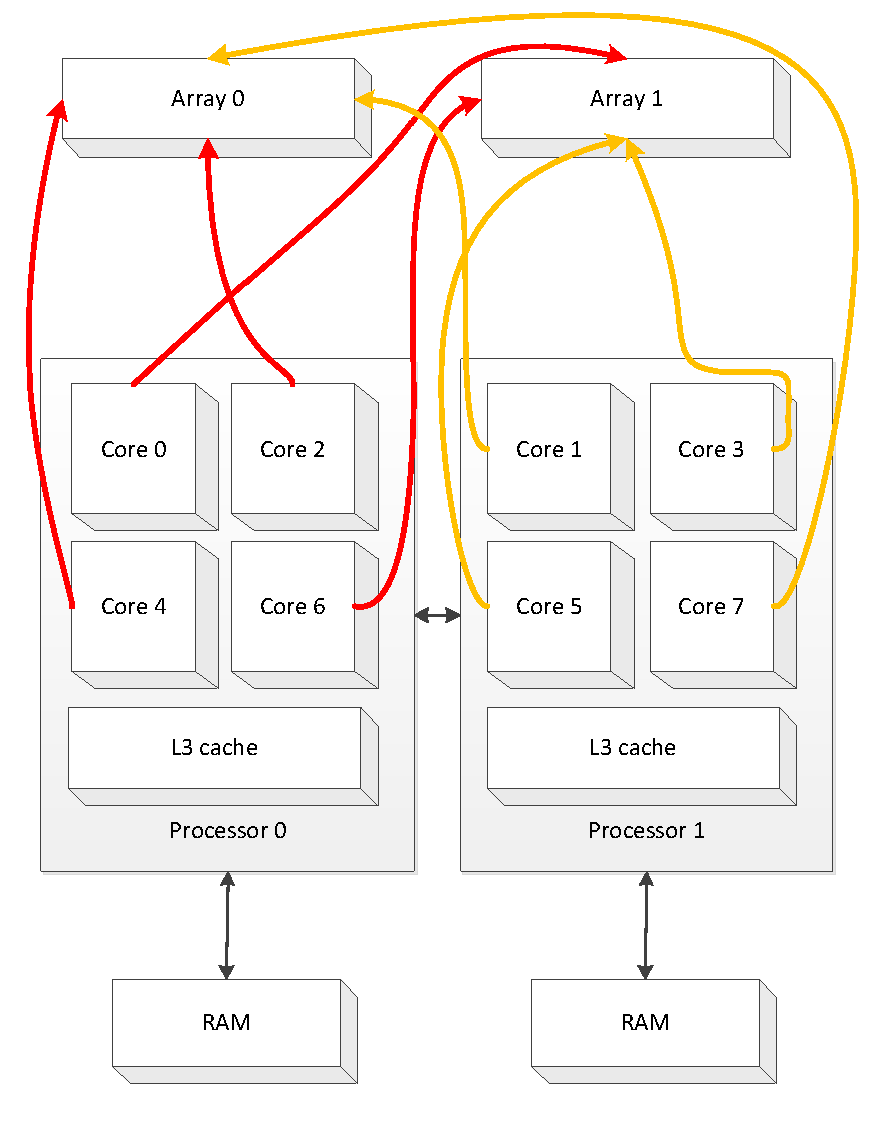
\includegraphics[width=0.5\linewidth]{locality-performance/cache-stress-test-mafushi-worst}
    \label{fig:locality-performance-cache-stress-mafushi-worst}
  }
  \caption{\emph{Cache Stress Test} with \emph{best} and \emph{worst
      locality}}
  \label{fig:locality-performance-cache-stress-test-mafushi}
\end{figure}

When running the intervals implementations of the \emph{Cache Stress
  Test} benchmarks, we observe similar behavior to the threaded
versions. As is shown in Table
\ref{tab:locality-performance-cache-stress-test} the implementation
with \emph{best locality} is the fastest and provides the largest
speedup.

\begin{table}[!htb]
  \centering
  \begin{tabular}{ln{2}{3}n{1}{2}}
    \toprule
    & {Runtime (in seconds)} & {Speedup (over sequential)} \\\midrule
    \emph{Best Locality} & 3.596 & 7.11 \\
    \emph{Ignorant Locality} & 4.038 & 6.33 \\
    \emph{Random Locality} & 4.030 & 6.35 \\
    \emph{Worst Locality} & 3.982 & 6.42 \\
    \emph{Sequential Implementation}\hspace{0.5cm} & 25.571 & 1 \\\bottomrule
  \end{tabular}
  \caption[\emph{Cache Stress Test} execution times]{\emph{Cache Stress Test} execution times and speedups over the sequential implementation}
  \label{tab:locality-performance-cache-stress-test}
\end{table}

In Figure \ref{fig:locality-performance-cache-stress-test} we show the
execution times normalized to that of the \emph{best locality}
implementation. The \emph{best locality} implementation is more than
10\% faster compared to the other locality benchmarks.

\begin{figure}[!ht]
  \centering
  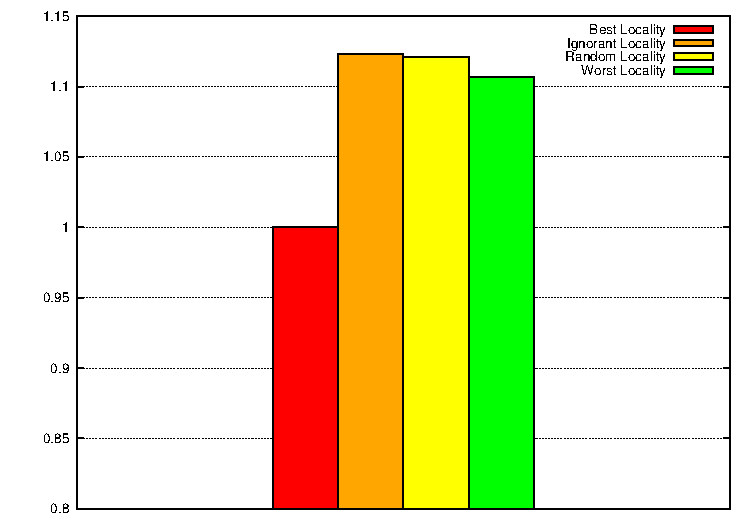
\includegraphics[width=0.8\linewidth]{locality-performance/cache-stress-test}
  \caption[\emph{Cache Stress Test} execution times]{\emph{Cache
      Stress Test} with execution times normalized to \emph{best
      locality}}
  \label{fig:locality-performance-cache-stress-test}
\end{figure}

In the \emph{best locality} benchmark, the intervals perform
prefetching of the array elements for one another. In the other
benchmarks, intervals compete for the L3 cache and overwrite one
another's entries. This reflects itself in the number of cache hit and
miss events listed in Table
\ref{tab:locality-performance-cache-stress-test-cache-hits-misses}.

\begin{table}[htb]
  \centering
  \begin{tabular}{ln{4}{0}n{4}{0}}
    \toprule
    & {L3 Cache Read Hits}  & {L3 Cache Read Misses} \\\midrule
    \emph{Best Locality}\hspace{1cm} & 2335 & 275 \\
    \emph{Ignorant Locality} & 1568 & 837 \\
    \emph{Random Locality} & 1570 & 854 \\
    \emph{Worst Locality} & 1539 & 837 \\\bottomrule
  \end{tabular}
  \caption[\emph{Cache Stress Test} L3 cache read hits and misses]{\emph{Cache Stress Test} L3 cache read hits and misses (rounded to the nearest million)}
  \label{tab:locality-performance-cache-stress-test-cache-hits-misses}
\end{table}

Figure \ref{fig:locality-performance-cache-stress-test} shows the
cache hits and misses normalized to the measurements of the \emph{best
  locality} implementation. The \emph{best locality} benchmark has up
to 1.5\texttimes\ more L3 cache read hits and 3.1\texttimes\ fewer L3
cache read misses than the other benchmarks.

\begin{figure}[!ht]
  \centering
  \subfloat[L3 Cache Read Misses]{
    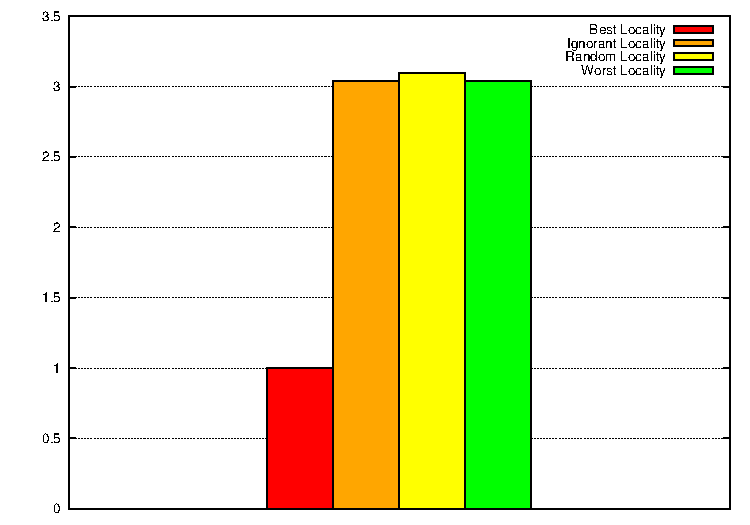
\includegraphics[width=0.66\linewidth]{locality-performance/cache-stress-test-cache-misses}
    \label{fig:locality-performance-cache-stress-test-cache-misses}
  }
  \\
  \subfloat[L3 Cache Read Hits]{
    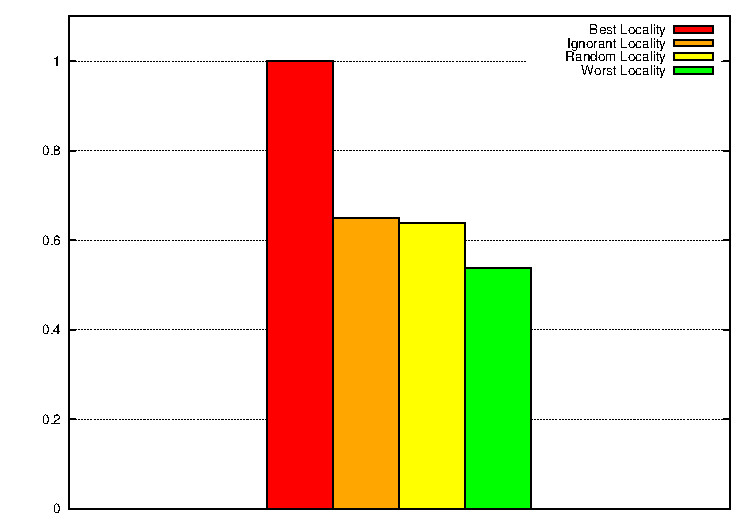
\includegraphics[width=0.66\linewidth]{locality-performance/cache-stress-test-cache-hits}
    \label{fig:locality-performance-cache-stress-test-cache-hits}
  }
  \caption[\emph{Cache Stress Test} L3 cache read hits and
  misses]{\emph{Cache Stress Test} with L3 cache read hits and misses
    normalized to \emph{best locality}}
  \label{fig:locality-performance-cache-stress-test-cache}
\end{figure}

The intervals implementation of the benchmarks with \emph{ignorant},
\emph{random} and \emph{worst locality} is faster compared to the
multi-threaded benchmark implementations of the same
localities. 

A reason for this is the use of \emph{Work-Stealing Places}. They have
a positive effect on the runtime due to their load-balancing
properties. As the number of cache hits and misses shows, they do not
produce counter-productive steals for the \emph{Cache Stress Test}
benchmarks.

\subsection{Merge Sort}
\label{sec:locality-performance-merge-sort}

The \emph{Merge Sort} benchmark uses divide-and-conquer to recursively
sort \numprint{4194304} randomly initialized integer values. Those
integers need about 16 MB of memory which is equal to the size of the
last level caches of our test machine.

\emph{Merge Sort} first creates \numprint{8192} sorter intervals per
worker, i.e. $8 \times \numprint{8192}$ sorters overall. Each sorter
randomly initializes an array of size $\numprint{4194304} / (8 \times
\numprint{8192})$ and sorts it with \lstinline!Arrays.sort()!. Merger
intervals merge two neighboring sorted arrays into one sorted array of
doubled size until all subarrays are merged into a large array of size
\numprint{4194304}. Figure
\ref{fig:locality-performance-mergesort-best-locality} shows an
example of the tree-like hierarchy of sorter and merger intervals used
to sort a randomly initialized list of integers with the help of 8
sorters and 7 mergers.

We implement several variants of the benchmark, each having different
locality properties:

\begin{description}
\item[Best Locality:] Half the sorter intervals have locality for
  \emph{place 0} and the other half have their locality set for
  \emph{place 1}. Merger intervals copy the locality of the interval
  they get the left array to merge from, i.e. they are scheduled on
  the same place as their left predecessors in the tree hierarchy.
\item[Ignorant Locality:] The sorter and merger intervals do not have
  any locality set, i.e. they are locality-ignorant.
\item[Worst Locality:] The sorter intervals have the same locality as
  in the \emph{best locality} implementation. The merger intervals set
  their locality to the other place as their left predecessor in the
  tree hierarchy, i.e. if the left predecessor was scheduled on
  \emph{place 0}, then the merger is scheduled on \emph{place 1} and
  vice versa.
\end{description}

Figure \ref{fig:locality-performance-mergesort-best-locality} shows
the place allocations for the benchmark variant with \emph{best
  locality}.

\begin{figure}[!ht]
  \centering
  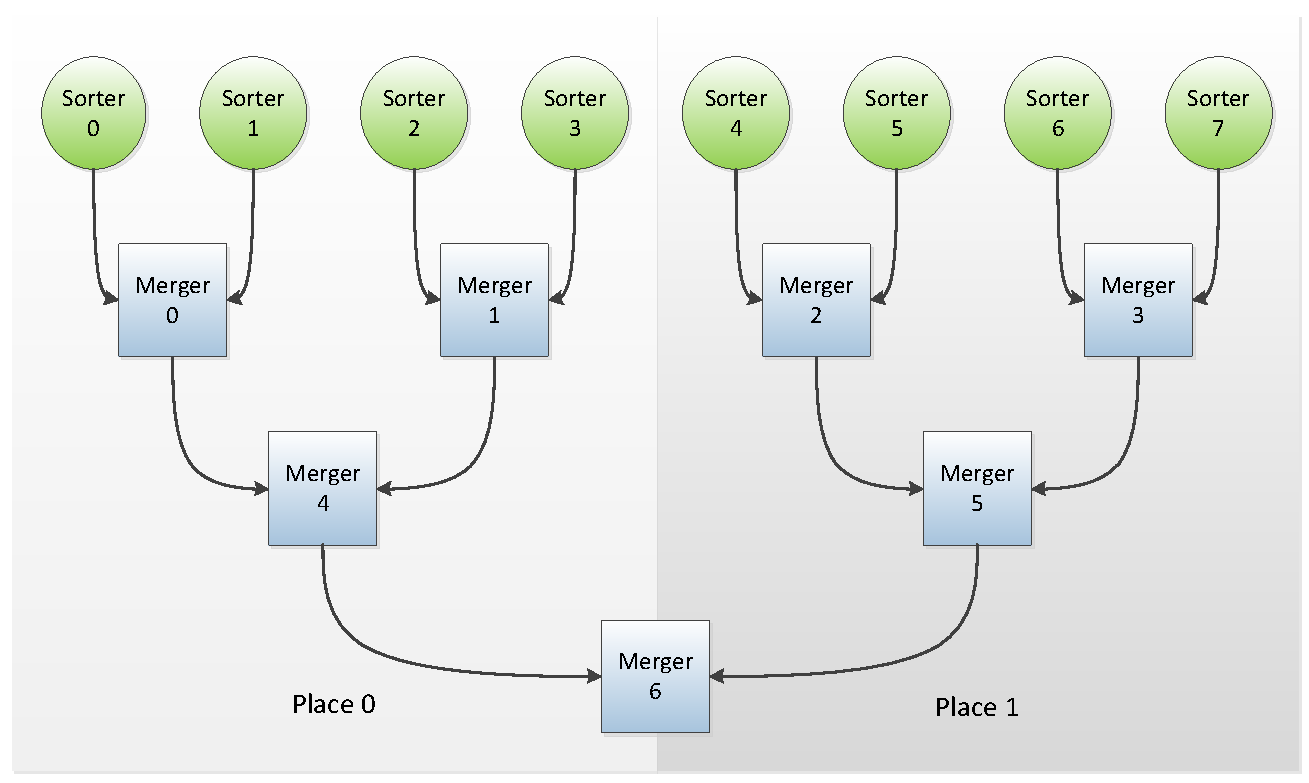
\includegraphics[width=\linewidth]{locality-performance/mergesort-best-locality}
  \caption{\emph{Merge Sort} with \emph{best locality}}
  \label{fig:locality-performance-mergesort-best-locality}
\end{figure}

The \emph{best locality} implementation puts data sharing intervals
onto the same \emph{place}. They perform prefetching for each other,
i.e. they help to obtain and maintain the frequently used integers in
the local L3 cache. With the \emph{worst locality} we try to achieve
the opposite: Merger intervals compete for the L3 caches and overwrite
each other's entries.

Table \ref{tab:locality-performance-mergesort} shows the execution
times and the speedups over the \emph{ignorant locality}
implementation for the \emph{best} and \emph{worst locality}
implementations. As expected, the implementation with \emph{best
  locality} is the fastest and provides the largest speedup.

\begin{table}[!htb]
  \centering
  \begin{tabular}{ln{3}{3}n{1}{2}}
    \toprule
    & {Runtime (in ms)} & {Speedup (over \emph{worst locality})} \\\midrule
    \emph{Best Locality} & 672.667 & 1.10 \\
    \emph{Worst Locality} & 726 & 1.02 \\
    \emph{Ignorant Locality} & 741.333 & 1 \\\bottomrule
  \end{tabular}
  \caption[\emph{Merge Sort} execution times]{\emph{Merge Sort} execution times and speedups over the \emph{ignorant locality} implementation}
  \label{tab:locality-performance-mergesort}
\end{table}

Figure \ref{fig:locality-performance-mergesort} illustrates the
execution times normalized to that of the \emph{best locality}
implementation. The \emph{best locality} implementation provides a
speedup of up to $1.1\times$ compared to the other locality
benchmarks.

\begin{figure}[!ht]
  \centering
  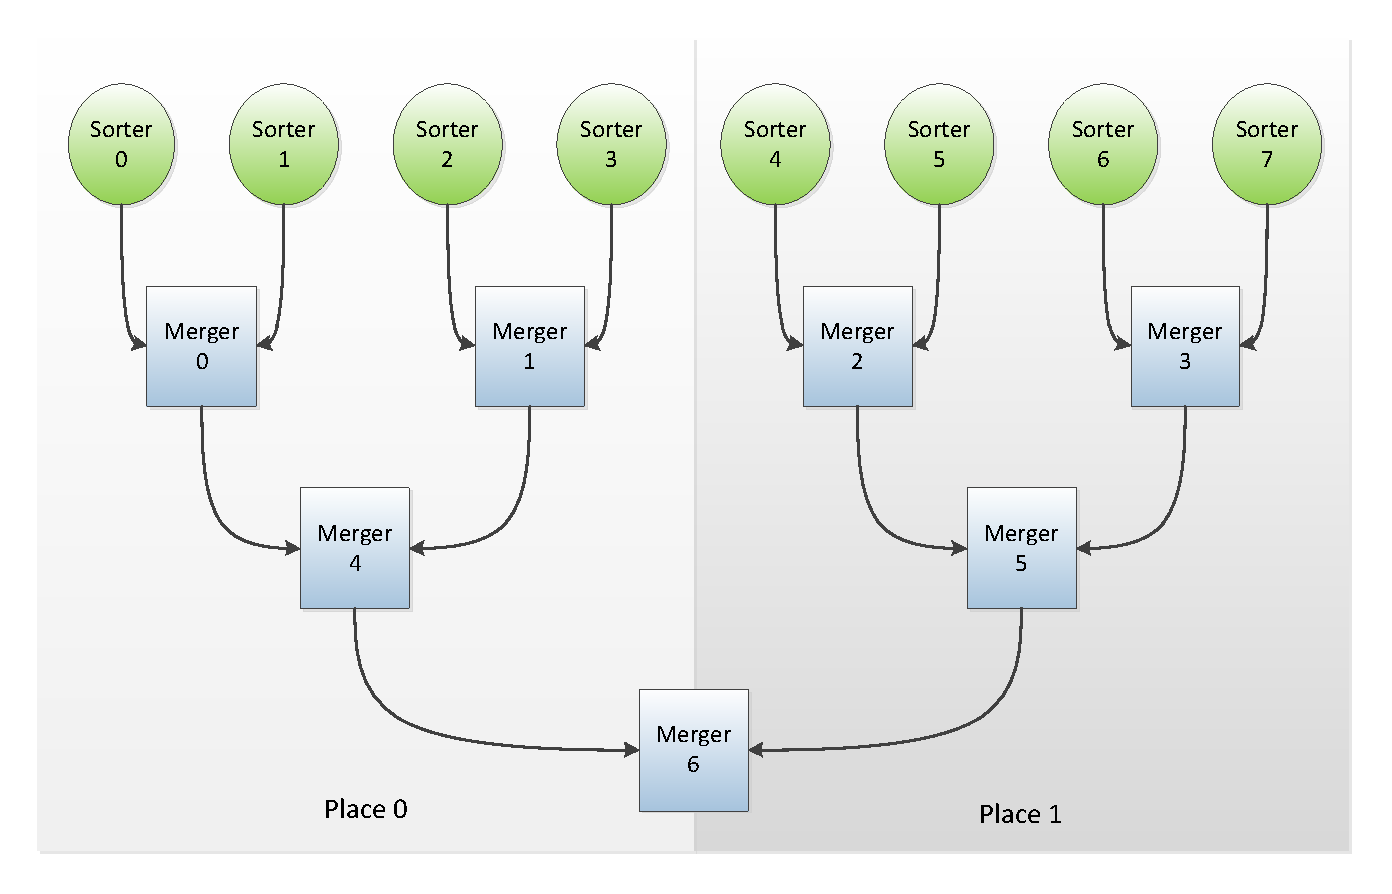
\includegraphics[width=0.8\linewidth]{locality-performance/mergesort}
  \caption[\emph{Merge Sort} execution times]{\emph{Merge Sort} with
    execution times normalized to \emph{best locality}}
  \label{fig:locality-performance-mergesort}
\end{figure}

In the \emph{best locality} benchmark, the intervals perform
prefetching of the array elements for one another. In the other
benchmarks, intervals compete for the L3 cache and overwrite each
other's entries. This reflects itself in the number of cache hit and
miss events listed in Table
\ref{tab:locality-performance-cache-stress-test-cache-hits-misses}.

\begin{table}[!htb]
  \centering
  \begin{tabular}{ln{4}{0}n{4}{0}}
    \toprule
    & {L3 Cache Read Hits}  & {L3 Cache Read Misses} \\\midrule
    \emph{Best Locality}\hspace{1cm} & 100 & 39 \\
    \emph{Worst Locality} & 99 & 41 \\
    \emph{Ignorant Locality} & 98 & 42 \\\bottomrule
  \end{tabular}
  \caption[\emph{Merge Sort} L3 cache read hits and misses]{\emph{Merge Sort} L3 cache read hits and misses (rounded to the nearest million)}
  \label{tab:locality-performance-cache-stress-test-cache-hits-misses}
\end{table}

The difference between the number of cache read hits and misses is
only marginal: The \emph{best locality} variant of the \emph{Merge
  Sort} benchmark has just about 2\% more cache read hits and 7\% less
cache read misses than the \emph{worst} and \emph{ignorant locality}
variants. This is mainly because of the rather small benchmark size
and limited level of data sharing between the intervals. Still, the
speedup of $1.1\times$ of the \emph{best locality} variant over the
\emph{ignorant locality} variant shows that last level cache misses
can have a significant impact on the runtime.


\subsection{Block Matrix Multiplication}
\label{sec:locality-performance-matmult}

The \emph{Block Matrix Multiplication} benchmark multiplies two $n
\times n$ matrices $A$ and $B$ using intervals. The implementation
employs the following recursion:

\begin{eqnarray*}
  \begin{pmatrix}
    C_{00} & C_{01} \\
    C_{10} & C_{11}
  \end{pmatrix}
  &
  =
  &
  \begin{pmatrix}
    A_{00} & A_{01} \\
    A_{10} & A_{11}
  \end{pmatrix}
  \cdot
  \begin{pmatrix}
    B_{00} & B_{01} \\
    B_{10} & B_{11}
  \end{pmatrix}
  \\[0.1cm]
  &
  =
  &
  \begin{pmatrix}
    A_{00} \cdot B_{00} + A_{01} \cdot B_{10} & A_{00} \cdot B_{01} + A_{01} \cdot B_{11} \\
    A_{10} \cdot B_{00} + A_{11} \cdot B_{10} & A_{10} \cdot B_{01} + A_{11} \cdot B_{11} \\
  \end{pmatrix}
\end{eqnarray*}

\vspace{0.1cm}

Thus, the $n \times n$ matrix multiplication can be reduced to 8
multiplications and 4 additions of $(n/2) \times (n/2)$
submatrices. The 8 multiplications can be calculated in parallel and
when they are done, the 4 additions can also be computed in parallel.

We run the \emph{Block Matrix Multiplication} benchmark to multiply
two random $2048 \times 2048$ matrices. A $2048 \times 2048$ matrix
needs about 16 MB of memory and should just about fit in the L3 cache
of the two processors of our test machine. 

The algorithm recursively splits the matrices $A$ and $B$ into
quadrants until the base case of size $32 \times 32$ is reached
(Figure \ref{fig:locality-performance-matmult-quadrants}). Then it
multiplies the corresponding $32 \times 32$ submatrices of $A$ and $B$
using sequential matrix multiplication to add them up.

\begin{figure}[!ht]
  \centering
  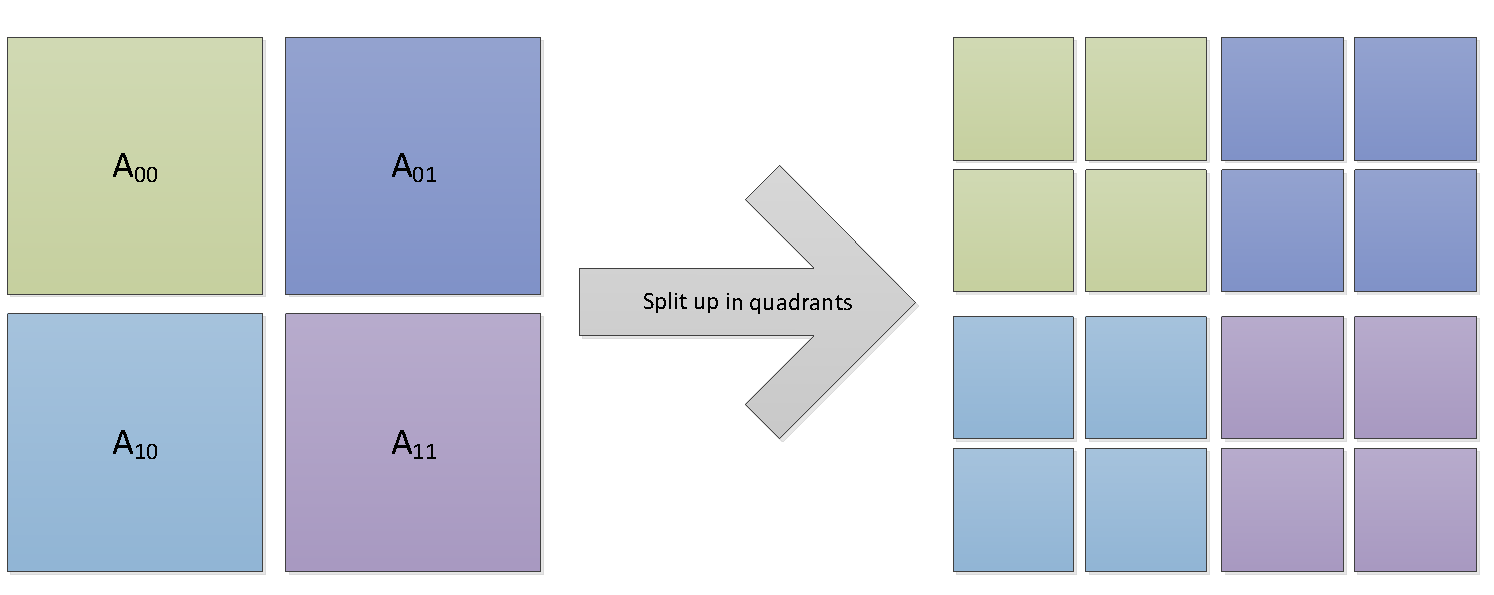
\includegraphics[width=0.88\linewidth]{locality-performance/matmult-quadrants}
  \caption{Splitting matrix $A$ into quadrants}
  \label{fig:locality-performance-matmult-quadrants}
\end{figure}

We implement two variants of the benchmark, \emph{best locality} and
\emph{worst locality}:

\begin{description}
\item[Best Locality:] The \emph{best locality} benchmark runs all
  addition and multiplication intervals of the submatrices of
  quadrants 0 and 3 in \emph{place 0} and the ones of the quadrants 1
  and 2 in \emph{place 1}. This way the places are able to share their
  local L3 cache in an efficient way.
\item[Worst Locality:] The \emph{worst locality} benchmark runs the
  multiplication and addition intervals in different places,
  destroying cache locality.
\end{description}

Figure \ref{fig:locality-performance-matmult-locality} illustrates the
division of matrix quadrants between places for both variants.

\begin{figure}[!ht]
  \centering
  \subfloat[Best Locality]{
    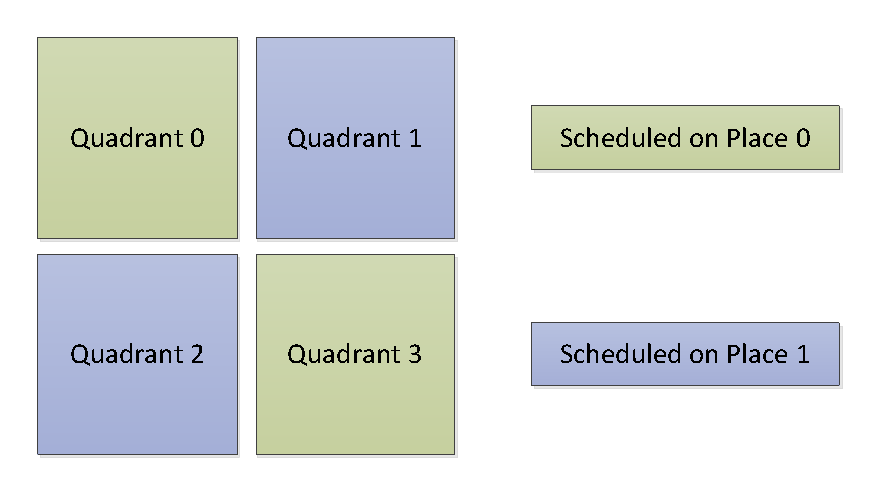
\includegraphics[width=0.55\linewidth]{locality-performance/matmult-best-locality}
    \label{fig:locality-performance-matmult-best-locality}
  }
  \\
  \subfloat[Worst Locality]{
    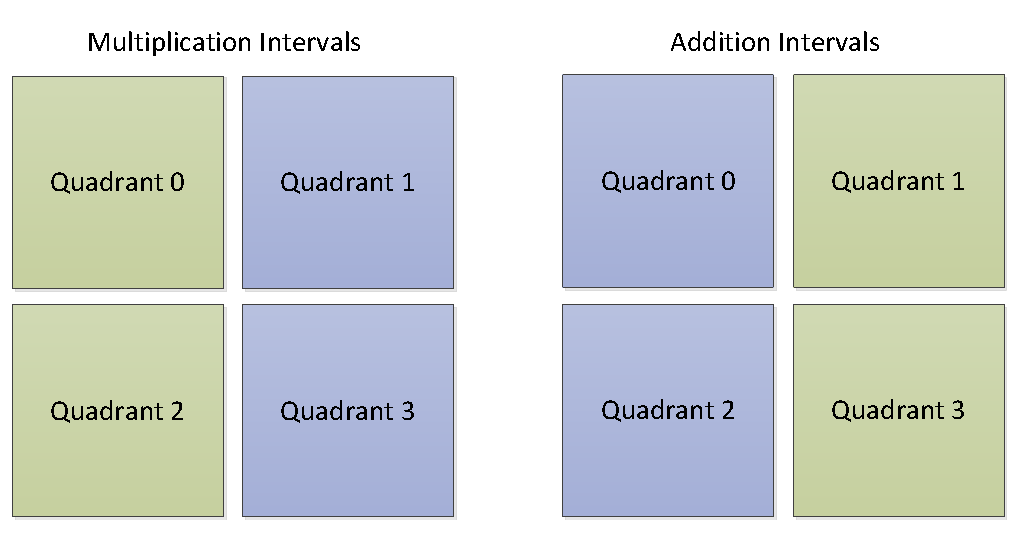
\includegraphics[width=0.6\linewidth]{locality-performance/matmult-worst-locality}
    \label{fig:locality-performance-matmult-worst-locality}
  }
  \caption{\emph{Block Matrix Multiplication} quadrants with \emph{best} and \emph{worst locality}}
  \label{fig:locality-performance-matmult-locality}
\end{figure}

Table \ref{tab:locality-performance-matmult} shows the execution times
and the speedups over the sequential algorithm for the \emph{best
  locality} and \emph{worst locality} benchmark implementations. As
expected, the implementation with \emph{best locality} is faster than
the one for the \emph{worst locality}.

\begin{table}[!htb]
  \centering
  \begin{tabular}{ln{2}{3}n{1}{2}}
    \toprule
    & {Runtime (in seconds)} & {Speedup (over sequential)} \\\midrule
    \emph{Best Locality} & 4.724 & 3.96 \\
    \emph{Worst Locality} & 5.075 & 3.69 \\
    \emph{Sequential Implementation}\hspace{0.5cm} & 18.703 & 1 \\\bottomrule
  \end{tabular}
  \caption[\emph{Block Matrix Multiplication} execution times]{\emph{Block Matrix Multiplication} execution times and speedups over the sequential implementation}
  \label{tab:locality-performance-matmult}
\end{table}

Figure \ref{fig:locality-performance-matmult} depicts the execution
time of the \emph{worst locality} implementation normalized to that of
the \emph{best locality} implementation. The \emph{best locality}
implementation shows a speedup over the \emph{worst locality} of about
1.07\texttimes.

\begin{figure}[!ht]
  \centering
  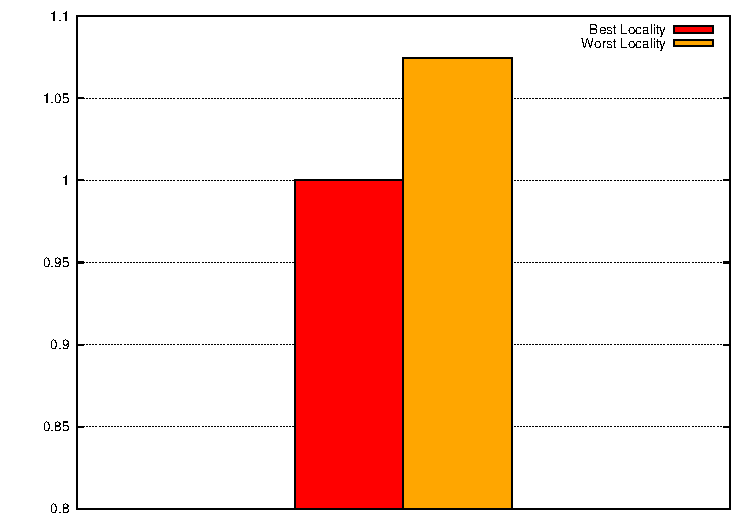
\includegraphics[width=0.7\linewidth]{locality-performance/matmult}
  \caption[\emph{Block Matrix Multiplication} execution
  times]{\emph{Block Matrix Multiplication} with execution times
    normalized to \emph{best locality}}
  \label{fig:locality-performance-matmult}
\end{figure}

The difference between the number of cache read hits and misses is
little (Table
\ref{tab:locality-performance-matmult-cache-hits-misses}): The
\emph{best locality} variant has just about 2\% more cache read hits
and 6\% less cache read misses than the \emph{worst locality}
variant. The main reason for this is the rather small benchmark size
and limited level of data sharing between the intervals. Last level
cache misses can have a significant impact on the runtime nevertheless
as is shown by the speedup of $1.07\times$ of the \emph{best locality}
variant over the \emph{worst locality}.

\begin{table}[!htb]
  \centering
  \begin{tabular}{ln{4}{0}n{4}{0}}
    \toprule
     & {L3 Cache Read Hits} & {L3 Cache Read Misses} \\\midrule
    \emph{Best Locality}\hspace{1cm} & 1283  & 352 \\
    \emph{Worst Locality} & 1256 & 374 \\\bottomrule
  \end{tabular}
  \caption[\emph{Merge Sort} L3 cache read hits and misses]{\emph{Block Matrix Multiplication} L3 cache read hits and misses (rounded to the nearest million)}
  \label{tab:locality-performance-matmult-cache-hits-misses}
\end{table}

%%% Local Variables: 
%%% mode: latex
%%% TeX-master: "thesis"
%%% End: 
